\documentclass{VUMIFPSkursinis}
\usepackage{algorithmicx}
\usepackage{algorithm}
\usepackage{algpseudocode}
\usepackage{amsfonts}
\usepackage{amsmath}
\usepackage{bm}
\usepackage{caption}
\usepackage{color}
\usepackage{float}
\usepackage{graphicx}
\usepackage{listings}
\usepackage{subfig}
\usepackage{wrapfig}

% Titulinio aprašas
\university{Vilniaus universitetas}
\faculty{Matematikos ir informatikos fakultetas}
\institute{Informatikos institutas}  % Užkomentavus šią eilutę - institutas neįtraukiamas į titulinį
\department{Programų sistemų studijų programa}
\papertype{Kursinis darbas}
\title{Vaizdo žaidimo eismo vaizdų generavimas naudojant nesuporuotų nuotraukų vertimą}
\titleineng{Video game traffic image generation using unpaired image to image translation}
\status{4 kurso 5 grupės studentas}
\author{Gytis Oksas}
\supervisor{j. asist. Boleslovas Dapkūnas}
\date{Vilnius – \the\year}

% Nustatymai
% \setmainfont{Palemonas}   % Pakeisti teksto šriftą į Palemonas (turi būti įdiegtas sistemoje)
\bibliography{bibliografija}

\begin{document}
\maketitle

\tableofcontents

\section{Įvadas}
%Įvade apibūdinamas darbo tikslas, temos aktualumas ir siekiami rezultatai. Darbo įvadas neturi būti dėstymo santrauka. Įvado apimtis 1–2 puslapiai.
Nuotraukų generavimas yra labai aktyvi ir greitai plėtojama giliųjų neuroninių tinklų sritis. Giliųjų neuroninių tinklų pritaikymas vaizdo žaidimuose ar jų meniniame turinyje yra nepaneigiamas. 2018 metais išėjęs straipsnis transformuojantis žaidimo Grand Theft Auto V (*įklijuoti straipsnį*) vaizdus į fotorealistinius tik įrodo, jog sekantis žingsnis į dar įtikinamesnius vaizdo žaidimų vaizdus yra gilieji neuroniniai tinklai. Tačiau yra atveju, kai norima eiti priešinga linkme - norima iš realistinių vaizdų sukurti jų atitikmenis tam tikrame meniniame domene (pvz. žmonių nuotraukų perkūrimas, kaip anime stiliumi *įklijuot straipsnį*). Taip greičiau ir patogiau kurti žaidimų meninį turinį gali padėti gilieji neuroniai tinklai. 

Šio tyrimo tikslas ir yra - sukurti modelį, kuris sugebėtų generuoti tam tikro žaidimo vaizdus iš jų norimo realistinio atitikmens, šiame tyrime buvo pasirinkta kurti žaidimo Grand Theft Auto: Vice City (toliau trumpinama "GTA:VC") domenas dėl jo išskirtinio meninio stiliaus ir ryškaus domeno požymių skirtumo lyginant su realaus eismo nuotraukomis.

Tyrimo siektinas rezultatas buvo sukurti modelį, kuris pasiektų FID įvertį žemesnį nei 100 (*įterpti straipsnį*), vizualiai būtų kuo artimesnis žaidimo vaizdams ir būtų praradęs kuo mažiau tikrų nuotraukų detalių.

\section{Duomenų rinkiniai}
\subsection{Naudojami duomenų rinkiniai}
Vaizdų transformavimui iš realistinių į GTA:VC vaizdus reikėjo dviejų duomenų rinkinių: realaus eismo vaizdų ir žaidimo eismo vaizdų. Realiaus eismo vaizdų duomenų rinkinių yra pakankamai daug, todėl jų rinkti nereikėjo ir buvo pasirinktas bdd100k rinkinys, o GTA:VC vaizdams reikėjo kurti savo duomenų rinkinį, kadangi kokybiško ir kiekybiško rinkinio internete rasti nepavyko. 
\subsection{Realistinių vaizdų duomenų rinkinys}
Kaip minėta, buvo naudojamas bdd100k duomenų rinkinys. Jis sudarytas iš 100 tūkst. automobilių eismo nuotraukų, padarytų naudojant kameras nukreiptas į automobilio važiavimo kryptį ir yra dažniausiai ant automobilio priekinės panelės. Buvo naudotas jo poaibis sudarytas iš 10 tūkst. nuotraukų, kadangi GTA:VC nuotraukų duomenų rinkinys gavosi lygintinai mažas. 10 tūkst. nuotraukų duomenų rinkinys yra padalintas 70:20:10 santykiu mokymui, testavimui ir validacijai (atitinkamai gaunasi 7 tūkst, 2 tūkst ir 1 tūkst). Kiekviena nuotrauka yra 1280:720 pikselių raiškos.

Papildomo apdorojimo ar modifikacijų duomenų rinkiniui nereikėjo, išskyrus paprasčiausią direktorijų keitimą ir aplankų pervadinimą, jog modelio treniravimo algoritmas žinotų, kur tiksliai rasti šaltinio domeno duomenų rinkinį.
\subsection{Grand Theft Auto: Vice City duomenų rinkinys}
Eksperimentą daryti buvo norima su GTA:VC vaizdais, tačiau jo duomenų rinkinio internete rasti nepavyko, todėl teko jį sukurti. Džiugu, jog kokybišką ir kiekybišką duomenų rinkinį leido sukurti žaidimo grafiniai nustatymai, todėl papildomų modifikacijų į žaidimą diegti nereikėjo, vienintelis dalykas, ko prireikė - ekrano vaizdo įrašymo programinės įrangos. Ekrano vaizdo įrašymui naudojama buvo OBS Studio programa.

OBS Studio programos paruošimo nereikėjo, bet buvo pakeistos kelios parinktys, kad kuriamas duomenų rinkinys būtų struktūriškai kuo panašesnis į šaltinio duomenų rinkinį ir vaizdo įrašai nesigautų be reikalo dideli ir sunkūs apdoroti. Pirma pakeista parinktis buvo pakeista raiška į bdd100k rinkinio nuotraukų raišką (kuri yra 1280:720 pikselių). Antras pakeitimas buvo nustatyti vaizdo įrašų kadrų dažnį kiekį į 1 kadrą per sekundę. Su paskutine parinktimi supaprastiname vaizdo įrašų perdarymą į nuotraukas, nes nereikia išmesti perteklinių nuotraukų nustačius didesnį kadrų dažnį (pvz. nustačius standartinius 60 kadrų per sekundę, gautume žymiai per daug nuotraukų).

GTA:VC žaidimui reikėjo kelių vaizdinių pakeitimų tam, kad būtų švaresni vaizdai ir būtų struktūriškai panašesnis į bdd100k duomenų rinkinį. Naudojant standartinius nustatymus yra rodomas vaizdas trečiuoju asmeniu (t.y. iš žaidėjo galo), apatiniame kairiajame kampe yra rodomas mažas žemėlapis ir viršuj dešinėje yra rodomi žaidimo duomenys: laikas, pinigai, gyvybės taškai, šarvų taškai, esami ginklai ir aktyvumas, kuriuo policija ieško žaidėjo (žr 1 pav.). Tam, kad vaizdas būtų artimesnis šaltinio domeno duomenų rinkiniui, reikėjo panaikinti žemėlapį ir informacines detales, tą žaidimas leido nustatymuose bei reikėjo nustatyti pirmą asmenį ir automobilio perspektyvos, kad nesimatytų pačio veikėjo ir taip išvengti nenorimų artefaktų (panašiai kaip įprastai lieka naudojant **dataset kur su mercedes** duomenų rinkinį, jame filmuojamas vaizdas iš automobilio Mercedes, o kadangi vaizduose yra matomas automobilio kapotas prie kurio pritvirtinta ikoniška Mercedes žvaigždė, todėl daugelyje transformuotų nuotraukų atsiranda minėtoji Mercedes žvaigždė). Šį pakeitimą žaidimas taip pat leidžia daryti, kaip konfiguracinį nustatymą. Šiuos pakeitimus implementavus, gaunamas kokybiškas ir švarus vaizdas, kuris nepalieka artefaktų ir užfiksuoja esminį turinį (žr. 2 pav.).
\begin{figure}[H]
    \centering
    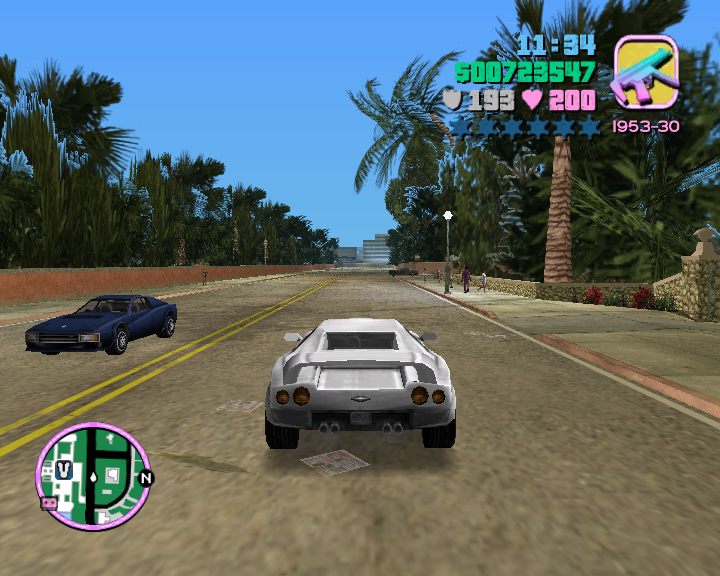
\includegraphics[scale=0.5]{img/neapdorotas_pvz}
    \caption{GTA:VC žaidimo vaizdas su įprastais nustatymais}
    \label{img:mlp}
\end{figure}
\begin{figure}[H]
    \centering
    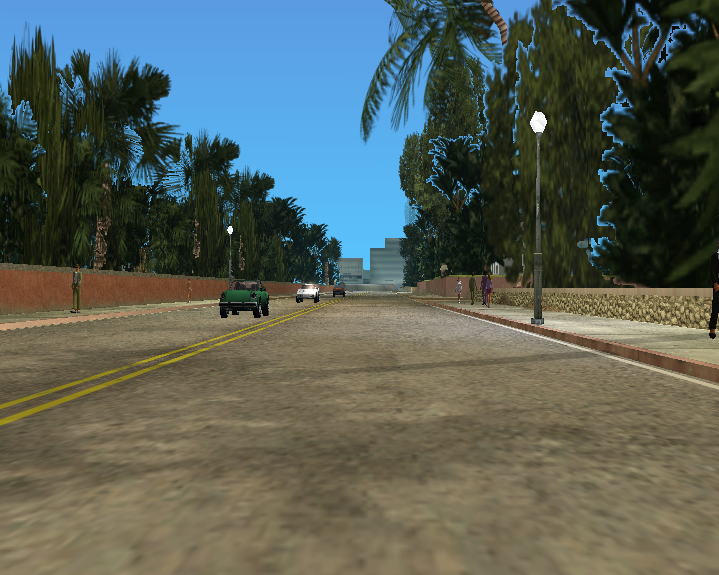
\includegraphics[scale=0.5]{img/apdorotas_pvz}
    \caption{GTA:VC žaidimo vaizdas su pakeistais nustatymais}
    \label{img:mlp}
\end{figure}

Duomenų rinkinio nuotraukos buvo kuriamos įrašinėjant GTA:VC žaidimo vaizdą, įrašuose važinėjant po žaidimo erdves keliais, bandant padengti kuo daugiau esamų vaizdų. Tas buvo daryta tiek žaidimo dienos metu, tiek nakties, kad būtų sukuriamas duomenų rinkinio aplinkybių vienodumas ir įvairumas. Žaidimo Pasaulis yra suskirstytas į 8 regionus. Kiekvienas regionas buvo išvažinėtas ir nufilmuotas žaidimo dienos ir nakties metu.

Kitame skyriuje yra minima, jog rezultatuose yra pastebėta spragų - vaizdai turi žymiai mažiau automobilių nuotraukose nei bdd100k duomenų rinkinys, todėl po kelių eksperimentų, reikėjo papildyti surinktą duomenų rinkinį nuotraukomis, kuriuose yra daug automobilių arba jie užima didesnį ekrano plotą. Tokių nuotraukų iš viso buvo padaryta 300 ir jas pridėjus prie kitų nuotraukų buvo sukurta antra duomenų rinkinio versija.

Visus regionus nufilmavus, jie buvo apdoroti Python kalbos skriptu, kuris vaizdo įrašo kadrus išskaidė į atskiras nuotraukas. Taip buvo iš viso sudaryta 2000 nuotraukų, o antra duomenų rinkinio versija buvo sudaryta iš 2300 nuotraukų.

\section{Parinkti modeliai}

\section{Modelių mokymas}

\section{Rezultatai}
\subsection{"Dingstančių automobilių problema"}


\end{document}
